\section{Link Modelling}\label{sec:linkmodel}
In this section, we propose a method for modelling and computing link \gls{pathloss} using building footprints
between nodes of a link, on OpenStreetMap map tiles obtained through the Mapbox Maps Service
API~\cite{website:mapbox}. The model computes the \gls{pathloss} based on the distance of the link and the
percentage of that distance that is in a building. Buildings and other environmental obstructions, which is
part of the shadow fading \gls{pathloss} from \cite{paper:linkmodel}, should cause a higher \gls{pathloss}, as
it is harder for the radio signal to propagate through buildings. \medbreak

The main idea is to generate a map of the area that contains nodes of a link as an image, and when computing
the \gls{pathloss} of that link, count the percentage of all pixels in a straight line between the nodes in a
link that are considered buildings on the map. The pseudo code description of this can be seen in
\autoref{algo:linkmodel:compute-building-percentage}.

%In this section, our own Linkmodel will be described.

%\subsection{Computing path loss}
%To facilitate to the problems discussed in \autoref{sec:reachi-experiments}, we have devised our own linkmodel
%to compute path loss. 
%Our model computes path loss based on the distance of the link and the percentage of
%that distance that is in a building. Building and other obstructions in the environment cause more severe path
%loss, and as such should be considered to punish the signal more. Our model limits to only buildings. 

%The idea
%is to generate a map of the area that the nodes are located in as an image, then when computing the path loss
%of a link, look up the colour of all pixels in a straight line between the nodes  of link and count how many
%is a building. This gives a percentage for how much of the distance is covered by buildings. An pseudo code
%implementation of the computation can be seen on \autoref{algo:linkmodel:compute-building-percentage}.

\begin{algorithm}[ht]
    \DontPrintSemicolon
    \KwIn{$(x_1, y_1), (x_2, y_2)$}
    \KwOut{Percentage building between points.}
    \SetKwFunction{FLoSModelCompute}{CompBuildingPct}
    \SetKwProg{Fn}{Function}{}{}

    \Fn{\FLoSModelCompute{$(x_1, y_1), (x_2, y_2)$}}{
        %$(n_1,\ n_2) \leftarrow \mathit{nodes}(l)$\;
        %$(x_1,\ y_1) \leftarrow$ compute position for $n_1$\;
        %$(x_2,\ y_2) \leftarrow$ compute position for $n_2$\;
        %\;
        $\mathit{pixels} \leftarrow 0$\;
        $\mathit{buildings} \leftarrow 0$\;
        \While{$\lambda \in \{0 \dots 1\}$}{
            $(x,\ y) \leftarrow \lambda \cdot (x_1,\ y_1) + (1 - \lambda)\cdot(x_2,y_2)$\;
            \If{position ($x$, $y$) is a building}{
                $\mathit{buildings} \leftarrow \mathit{buildings} + 1$\;
            }
            $\mathit{pixels} \leftarrow \mathit{pixels} + 1$\;
        }

        \KwRet $\frac{\mathit{buildings}}{\mathit{pixels}}$\;
    }
    \caption{The CompBuildingPct function.}
    \label{algo:linkmodel:compute-building-percentage}
\end{algorithm}

To compute the total \gls{pathloss}, we first define two functions: $\mathit{cvpl}(l)$ (\gls{cvpl}) and
$\mathit{bopl}(l)$ (\gls{bopl}). Both functions compute the distance-dependent \gls{pathloss}, similarly to
the $\mathit{pl}_d$ function from \autoref{sec:reachi-experiments}, but rather than computing the total
distance based \gls{pathloss}, we need to define a similar function for the distance with a clear view, and a
similar function to the distance where buildings obstruct the signal. To do this, we define this as an
optimisation problem, where we want to find the optimal constants for the two functions, by minimising the
difference between the computed \gls{rssi} and the measured \gls{rssi} for a set of links $L$. The
$\mathit{compRSSI}(l) = \mathit{tx}_\mathit{power} - (\alpha \cdot (\ln(d(l)) / \ln(\delta)) + \beta)$
function denotes the computed \gls{rssi} for a link with the chosen values for $\alpha$, $\beta$, and
$\delta$.
\medbreak

The problem is defined as follows:

\begin{itemize}
    \item Input: A set of links $L$.
    \item Output: Optimal values for $\alpha, \beta, \delta$.
    \item Goal: Minimise the $\mathit{score}(\alpha, \beta, \delta)$ function:

          $\mathit{score}(\alpha, \beta, \delta) = \mathlarger{\sum}\limits_{l \in L} (\mathit{compRSSI}(l) - \mathit{measuredRSSI}(l))^2$
\end{itemize}

\subsection{Greedy Approach}
To solve the optimisation problem, we have chosen a greedy approach. First, to compute the optimal values for
the $\mathit{cvpl}(l)$ function, we compile a set of links $L$, where the computed building percentage is
below 5 \%, and for the $\mathit{bopl}(l)$ function, we compile a set of links $L$ where the computed building
percentage is above 80 \%. Ideally, we would like for the building percentage to be close to 100 \%, but the
number of links in the Marikina log with more than 95 \% of buildings is very low. With these sets, we attempted
to find the optimal values for $\alpha$, $\beta$, and $\delta$ by going through $\alpha, \beta \in \{-100,
\dots, 100\}$ with increments of $0.5$, and $\delta \in \{2, \dots, 100\}$ with increments of $1$. This
resulted in the following values for the $\mathit{cvpl}(l)$ and $\mathit{bopl}(l)$ functions:
%
\begin{eq} 
    \mathit{cvpl}(l) = 48.5 \cdot (\ln{(d(l))} / \ln{(77)}) + 37.5 
\end{eq}

\begin{eq} 
    \mathit{bopl}(l) = 67 \cdot (\ln{(d(l))} / \ln{(57))} + 11.5 
\end{eq}


%To solve the optimisation problem, brute forcing will be utilised because of time restrictions. The set of
%links $L$, consisted of links with a computed building percentage below five percent or above 80\% was
%collected from the Marikina log into their separate collections. The Marikina log was used because the
%experiment was conducted in a city, resulting in links with varying building percentages. For both
%collections the links were further sorted based on distance of the links, with 20 meter intervals i.e. links
%with distances between 20 meters and 40 meters was sorted together. The average \gls{rssi} for each
%separation was then computed. Links with building percentage above 80\% was used for $\mathit{bopl}$ and
%links below 5 percent for $\mathit{cvpl}$. The parameters $\alpha,\ \beta \in \{-100 \dots 100\}$ with $0.5$
%increments and $\delta\ \in \{2 \dots 100\}$ with $1$ increments. The result was the following functions:
%\begin{eq} \mathit{cvpl}(l) = 48.5 \cdot (\ln{(d(l))} / \ln{(77)}) + 37.5 \end{eq}
%
%\begin{eq} \mathit{bopl}(l) = 67 \cdot (\ln{(d(l))} / \ln{(57))} + 11.5 \end{eq}


%We define two functions, $\mathit{cvpl}(l)$ and $\mathit{bopl}(l)$. Both functions compute path
%loss based on distance. \gls{cvpl} computes path loss for distances with zero percent building, while
%\gls{bopl} computes path loss for 100\% building. When computing the path loss both functions will be used, in
%the following equation:
%\todo[inline]{make me prettier}

%\todo[inline]{finish block}


%Finding the optimal constants for $\mathit{cvpl}$ and $\mathit{bopl}$ can defined as an optimisation problem.
%A set of links $L$ must be provided. The goal is to compute the difference from the computed \gls{rssi} to the
%measurements for all links in $L$.
%\medbreak

%The problem is defined as follows:
%\begin{itemize}
%    \item Input: A set of link $L$.
%    \item Output: Optimal parameters for $\alpha,\ \beta,\ \delta$.
%    \item Goal: Minimise the score function:\smallbreak
%    $\mathit{compRSSI}(l)= \alpha \cdot (log_\delta(d(l))) + \beta$\smallbreak
%    $\mathit{score}(\alpha, \beta, \delta) = \sum\limits_{l\ \in\ L} (\mathit{compRSSI}(l) - \mathit{measuredRSSI}(l))^2$
%
%\end{itemize}

With these two functions defined, we can compute the total \gls{pathloss} for a link. The function
$p(l)$ denotes the points for the links, as required by the input to the CompBuildingPct function.
%
\begin{eq}\label{eq:pl} %%% REMEMBER %%%
    \mathit{pl}(l) = (\mathit{cvpl}(l) \cdot (1 - \text{CompBuildingPct}(p(l)))) + (\mathit{bopl}(l) \cdot \text{CompBuildingPct}(p(l)))
\end{eq}

Finally, with the $\mathit{pl}(l)$ function, we can compute the \gls{rssi} for the link $l$: 
%
\begin{eq}\label{eq:plrssi}
    \mathit{RSSI}_{\mathit{dBm}}(l) = \mathit{tx}_\mathit{power} - \mathit{pl}(l)
\end{eq}

\subsection{Evaluation}

The functions $\mathit{cvpl}(l)$ and $\mathit{bopl}(l)$ have been plotted
on \autoref{plot:reachi-experiments:cvpl-vs-bopl}. $\mathit{bopl}$ do result in greater \gls{pathloss}, however,
the plot also reveals that up to 100 meters, $\mathit{bopl}(l)$ compute a better \gls{rssi} compared to
$\mathit{cvpl}(l)$. To further examine this, each function has been plotted with their training set.
$\mathit{cvpl}(l)$ on \autoref{plot:reachi-experiments:marikina-log-below-5-pct} and $\mathit{bopl}(l)$ can be
seen in \autoref{plot:reachi-experiments:marikina-log-above-80-pct}.

\begin{figure}[H]
    \centering
    \begin{tikzpicture}
        \begin{axis}[
                height=10cm, width=0.95\textwidth,
                ylabel={RSSI},
                xlabel={Distance in meters},
                axis lines*=left,
                xmin=0, xmax=750,
                enlargelimits=false,
                ymajorgrids=true,
                xmajorgrids=true,
                grid style=dashed,
                restrict y to domain=-120:0,
                samples=700
            ]

            \addplot[domain=0:1000, very thick, solid, cyan] {26 - bopl(x)};
            \addlegendentry{\gls{bopl}};

            \addplot[domain=0:1000, very thick, dashed, red] {26 - cvpl(x)};
            \addlegendentry{\gls{cvpl}};
        \end{axis}
    \end{tikzpicture}
    \caption{Plot showing samples drawn from \gls{cvpl} and \gls{bopl}}
    \label{plot:reachi-experiments:cvpl-vs-bopl}
\end{figure}

\begin{figure}[H]
    \centering
    \begin{tikzpicture}
        \begin{axis}[
                title={score: 501.4932, links: 13481, score/link: 0.0372},
                height=10cm, width=0.95\textwidth,
                ylabel={RSSI},
                xlabel={Distance in meters},
                axis lines*=left,
                xmin=0, xmax=750,
                enlargelimits=false,
                ymin=-90, ymax=-30,
                xtick={0, 50, 100, 150, 200, 250, 300, 350, 400, 450, 500, 550, 600, 650, 700, 750},
                ymajorgrids=true,
                xmajorgrids=true,
                grid style=dashed,
                samples=700
            ]

            \addplot[very thick, solid, cyan, mark=*] coordinates {(20, -36.01344537815126) (40, -48.361111111111114) (60, -54.93279022403259) (80, -62.40816326530612) (100, -68.14871794871794) (120, -60.85954712362301) (140, -71.69568452380952) (160, -74.36896551724138) (180, -73.93817204301075) (200, -75.09929078014184) (220, -73.38403041825094) (240, -75.43994413407822) (260, -77.69102990033223) (280, -77.31512605042016) (300, -75.7751937984496) (320, -78.60714285714286) (340, -78.38524590163935) (360, -78.52459016393442) (380, -77.34285714285714) (400, -80.96153846153847) (420, -81.03571428571429) (440, -80.41379310344827) (460, -74.18181818181819) (480, -79.9090909090909) (500, -79.75) (520, -77.56521739130434) (540, -81.23076923076923) (560, -78.9) (580, -85.0) (620, -82.5) (640, -82.33333333333333) (660, -82.4) (680, -77.5) (700, -85.4) (740, -77.0)};
            \addlegendentry{Marikina field measurements}


            \addplot[domain=0:740, very thick, solid, red] {26 - cvpl(x)};
            \addlegendentry{\gls{cvpl}};
        \end{axis}
    \end{tikzpicture}
    \caption{Field measurements with building percentage below 5 \%.}
    \label{plot:reachi-experiments:marikina-log-below-5-pct}
\end{figure}

\begin{figure}[H]
    \centering
    \begin{tikzpicture}
        \begin{axis}[
                title={score: 350.6854, links: 377, score/link: 0.9302},
                height=10cm, width=0.95\textwidth,
                ylabel={RSSI},
                xlabel={Distance in meters},
                axis lines*=left,
                xmin=0, xmax=380,
                enlargelimits=false,
                ymin=-90, ymax=-30,
                ymajorgrids=true,
                xmajorgrids=true,
                grid style=dashed,
                samples=400
            ]

            \addplot[very thick, solid, cyan, mark=*] coordinates {(20, -32.56521739130435) (40, -50.607142857142854) (60, -52.15384615384615) (80, -64.85714285714286) (100, -49.5) (120, -65.76623376623377) (140, -69.38888888888889) (160, -72.05714285714286) (180, -69.3125) (200, -78.83333333333333) (220, -76.84) (240, -75.75) (260, -80.91666666666667) (280, -72.88888888888889) (300, -78.95238095238095) (320, -76.44444444444444) (340, -82.75) (380, -87.0)};
            \addlegendentry{Marikina field measurements};

            \addplot[domain=0:380, very thick, solid, red] {26 - bopl(x)};
            \addlegendentry{\gls{bopl}};
        \end{axis}
    \end{tikzpicture}
    \caption{Field measurements with building percentage above 80 \%.}
    \label{plot:reachi-experiments:marikina-log-above-80-pct}
\end{figure}

With the optimal values for the $\mathit{cvpl}(l)$ function, the final score was 501.4932 for 13481 links with
less than 5 \% buildings. \autoref{plot:reachi-experiments:marikina-log-below-5-pct} shows how well this
function fits with the measured values. \smallbreak

For the $\mathit{bopl}(l)$ function, we got a final score of 350.6854 for 377 links with more than 80 \%
buildings. This is a very large difference compared to the 13481 links for the $\mathit{cvpl}(l)$, which means 
that we might experience lower precision for the $\mathit{bopl}(l)$ function.

%With the found optimal parameters for $\mathit{cvpl}$, the resulting was score was 501.4932 for 13481 links.
%The average score for a single link is then $0.0372 = 501.4932 / 13481$. We consider this as good score, and
%as can be seen on \autoref{plot:reachi-experiments:marikina-log-below-5-pct}, the function fits the
%measurements.\medbreak
%
%The $\mathit{bopl}$ however got worse result. The score per link was 0.9302 which is much larger compared to
%the score for $\mathit{cvpl}$. It is important to note that there was only 377 links in the training set for
%the $\mathit{bopl}$ function, which is vastly less compared to the 13481 links for the $\mathit{cvpl}$
%function. Another reason for the lower precision of $\mathit{bopl}$ is that the training set does not only
%consist of links with 100\% building, as we allowed for links with more than 80\%. This was however necessary
%as there was close to none links with 100\% building. Having a large set of links with 100\% building would
%result in higher precision.

Finally, a comparison of the computed \gls{rssi} values from \autoref{eq:plrssi} with the measurements from
the Marikina log is shown in \autoref{plot:reachi-experiments:marikina-log-vs-computed}. The plot shows that
the function is slightly off on the from about 75 meters to 300 meters, but compared to
\autoref{plot:reachi-experiments:measurements-vs-ld}, we do see an improvement.

\begin{figure}[ht]
    \centering
    \begin{subfigure}[b]{0.48\textwidth}
        \centering
        \qrcode[hyperlink]{https://youtu.be/vVqHzVThW34}
        \caption{Field measurements visualised.}
        \label{fig:field-measurements-visualised-qr}
    \end{subfigure}
    \hfill
    \begin{subfigure}[b]{0.48\textwidth}
        \centering
        \qrcode[hyperlink]{https://youtu.be/tZdhf6zcs2Y}
        \caption{Computed \gls{rssi} values visualised.}
        \label{fig:computed-values-visualised-qr}
    \end{subfigure}
    \caption{Marikina field measurements and computed \gls{rssi} values.}
    \label{fig:building-visualisation}
\end{figure}

\autoref{fig:building-visualisation} contains YouTube links to two visualisations, where 
\autoref{fig:field-measurements-visualised-qr} visualises the Marikina field measurements, and 
\autoref{fig:computed-values-visualised-qr} visualises the computed \gls{rssi} values. Both visualisations
highlight the same subset of the links, to make it easier to follow. \medbreak

The complete source code for the C++ implementation can be found on GitHub:

\url{https://github.com/Joklost/sims2}

\begin{figure}[H]
    \centering
    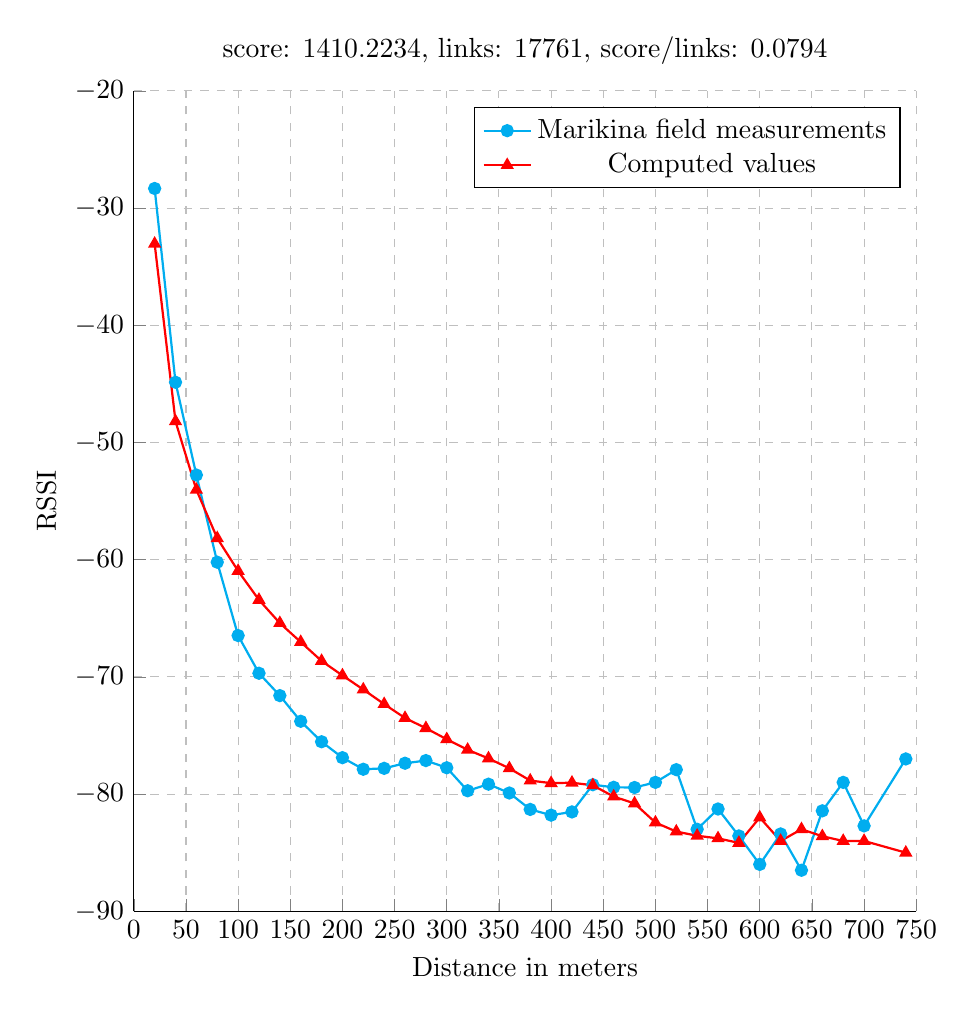
\begin{tikzpicture}
        \begin{axis}[
                title={score: 1410.2234, links: 17761, score/links: 0.0794},
                height=12cm, width=0.95\textwidth,
                ylabel={RSSI},
                xlabel={Distance in meters},
                axis lines*=left,
                xmin=0, xmax=750,
                enlargelimits=false,
                ymin=-90, ymax=-20,
                xtick={0, 50, 100, 150, 200, 250, 300, 350, 400, 450, 500, 550, 600, 650, 700, 750},
                ymajorgrids=true,
                xmajorgrids=true,
                grid style=dashed,
            ]

            \addplot[thick, solid, cyan, mark=*] coordinates {(20, -28.32345013477089) (40, -44.85830258302583) (60, -52.77323717948718) (80, -60.21201657458563) (100, -66.47435897435898) (120, -69.68905472636816) (140, -71.5976496922216) (160, -73.7866473149492) (180, -75.53428571428572) (200, -76.89289392378991) (220, -77.88135593220339) (240, -77.8035019455253) (260, -77.36784140969164) (280, -77.14030612244898) (300, -77.75299760191847) (320, -79.71686746987952) (340, -79.15481171548117) (360, -79.90728476821192) (380, -81.30909090909091) (400, -81.79746835443038) (420, -81.52272727272727) (440, -79.2) (460, -79.42105263157895) (480, -79.4375) (500, -79.0) (520, -77.91666666666667) (540, -83.0) (560, -81.27272727272727) (580, -83.57142857142857) (600, -86.0) (620, -83.4) (640, -86.5) (660, -81.42857142857143) (680, -79.0) (700, -82.71428571428571) (740, -77.0)};
            \addlegendentry{Marikina field measurements};

            \addplot[thick, solid, red, mark=triangle*] coordinates {(20,-33.04359925788497)(40,-48.19327731092437)(60,-54.03703703703704)(80,-58.16688567674113)(100,-60.96085858585859)(120,-63.43184421534937)(140,-65.41129831516353)(160,-67.02463054187191)(180,-68.64031007751937)(200,-69.87730061349693)(220,-71.07770961145194)(240,-72.32267441860465)(260,-73.50986842105263)(280,-74.37786259541984)(300,-75.32413793103449)(320,-76.22083333333333)(340,-76.95930232558139)(360,-77.8018018018018)(380,-78.84883720930233)(400,-79.06557377049181)(420,-79.03030303030303)(440,-79.25)(460,-80.21428571428571)(480,-80.8)(500,-82.42857142857143)(520,-83.2)(540,-83.55555555555556)(560,-83.77777777777777)(580,-84.16666666666667)(600,-82.0)(620,-84.0)(640,-83.0)(660,-83.6)(680,-84.0)(700,-84.0)(740,-85.0)};
            \addlegendentry{Computed values};
        \end{axis}
    \end{tikzpicture}
    \caption{Field measurements vs. computed values.}
    \label{plot:reachi-experiments:marikina-log-vs-computed}
\end{figure}

%Finally a comparison of the computed results from \autoref{eq:pl} compared with the measurements from the
%Marikina log. Once again, links have been sorted into distance buckets and had the average \gls{rssi} for each
%bucket computed. The computed \gls{rssi}, was computed with \autoref{eq:pl} on the links from the Marikina
%log, but the field measured \gls{rssi} was removed. The computed \gls{rssi} was added instead, and the same
%sorting into distance buckets was done with the computed log. The result can be seen on
%\autoref{plot:reachi-experiments:marikina-log-vs-computed}. The computed score, once again, for a single link
%was 0.0794. \autoref{plot:reachi-experiments:marikina-log-vs-computed} shows that the function is off on the
%range from about 75 meters to 300 meters, however when compared with
%\autoref{plot:reachi-experiments:measurements-vs-ld} ours does indeed give a better result.